\section{Results}


\section*{Discussion}
(Comment on your results, explain what those results mean, interpret the results in a wider context. Also indicate which results were expected or unexpected, and provide an explanation for the unexpected results)

\begin{comment}


\subsection{Grid vs graph connectivity}
Explain
\begin{itemize}
    \item both methods 
    \item that the graph doesn't work on weird buildings but grid system does.
    \item That grid scales badly with building size but graph doesn't
    \item f
    \item f
    \item f
    \item Maybe variation in node sizes help
    \item That the robot needs a certain node size to work properly. It doesn't work on nodes in the $mm^2$ range.
\end{itemize}


To make the robot walk from one room to another or one place in the building to another, it is important to understand the and decide on a way to implement the connectivity between the rooms. There are mainly two different kinds of implementations; a graph connectivity implementation and a grid implementation.
\\\\
The grid implementation works by discretizing the floor of the building into a grid with nodes of a specific size; the smaller the node size the higher the resolution of the grid.
\\
The graph connectivity approach works by representing each room/area by a node/dot which will be connected by a line to other rooms in the floor.

The different implementations have different advantages and limitations. For example computationally the graph connectivity approach is much more scalable with bigger buildings or construction sites where as implementing a grid system in these situations will be more taxing computationally since a lot of nodes will have to be calculated. 

On the other hand the advantage of the grid method is that its pathfinding algorithms will work on all building shapes. 
Imagine the floor plan of the building below:


\begin{figure}[H]
    \centering
    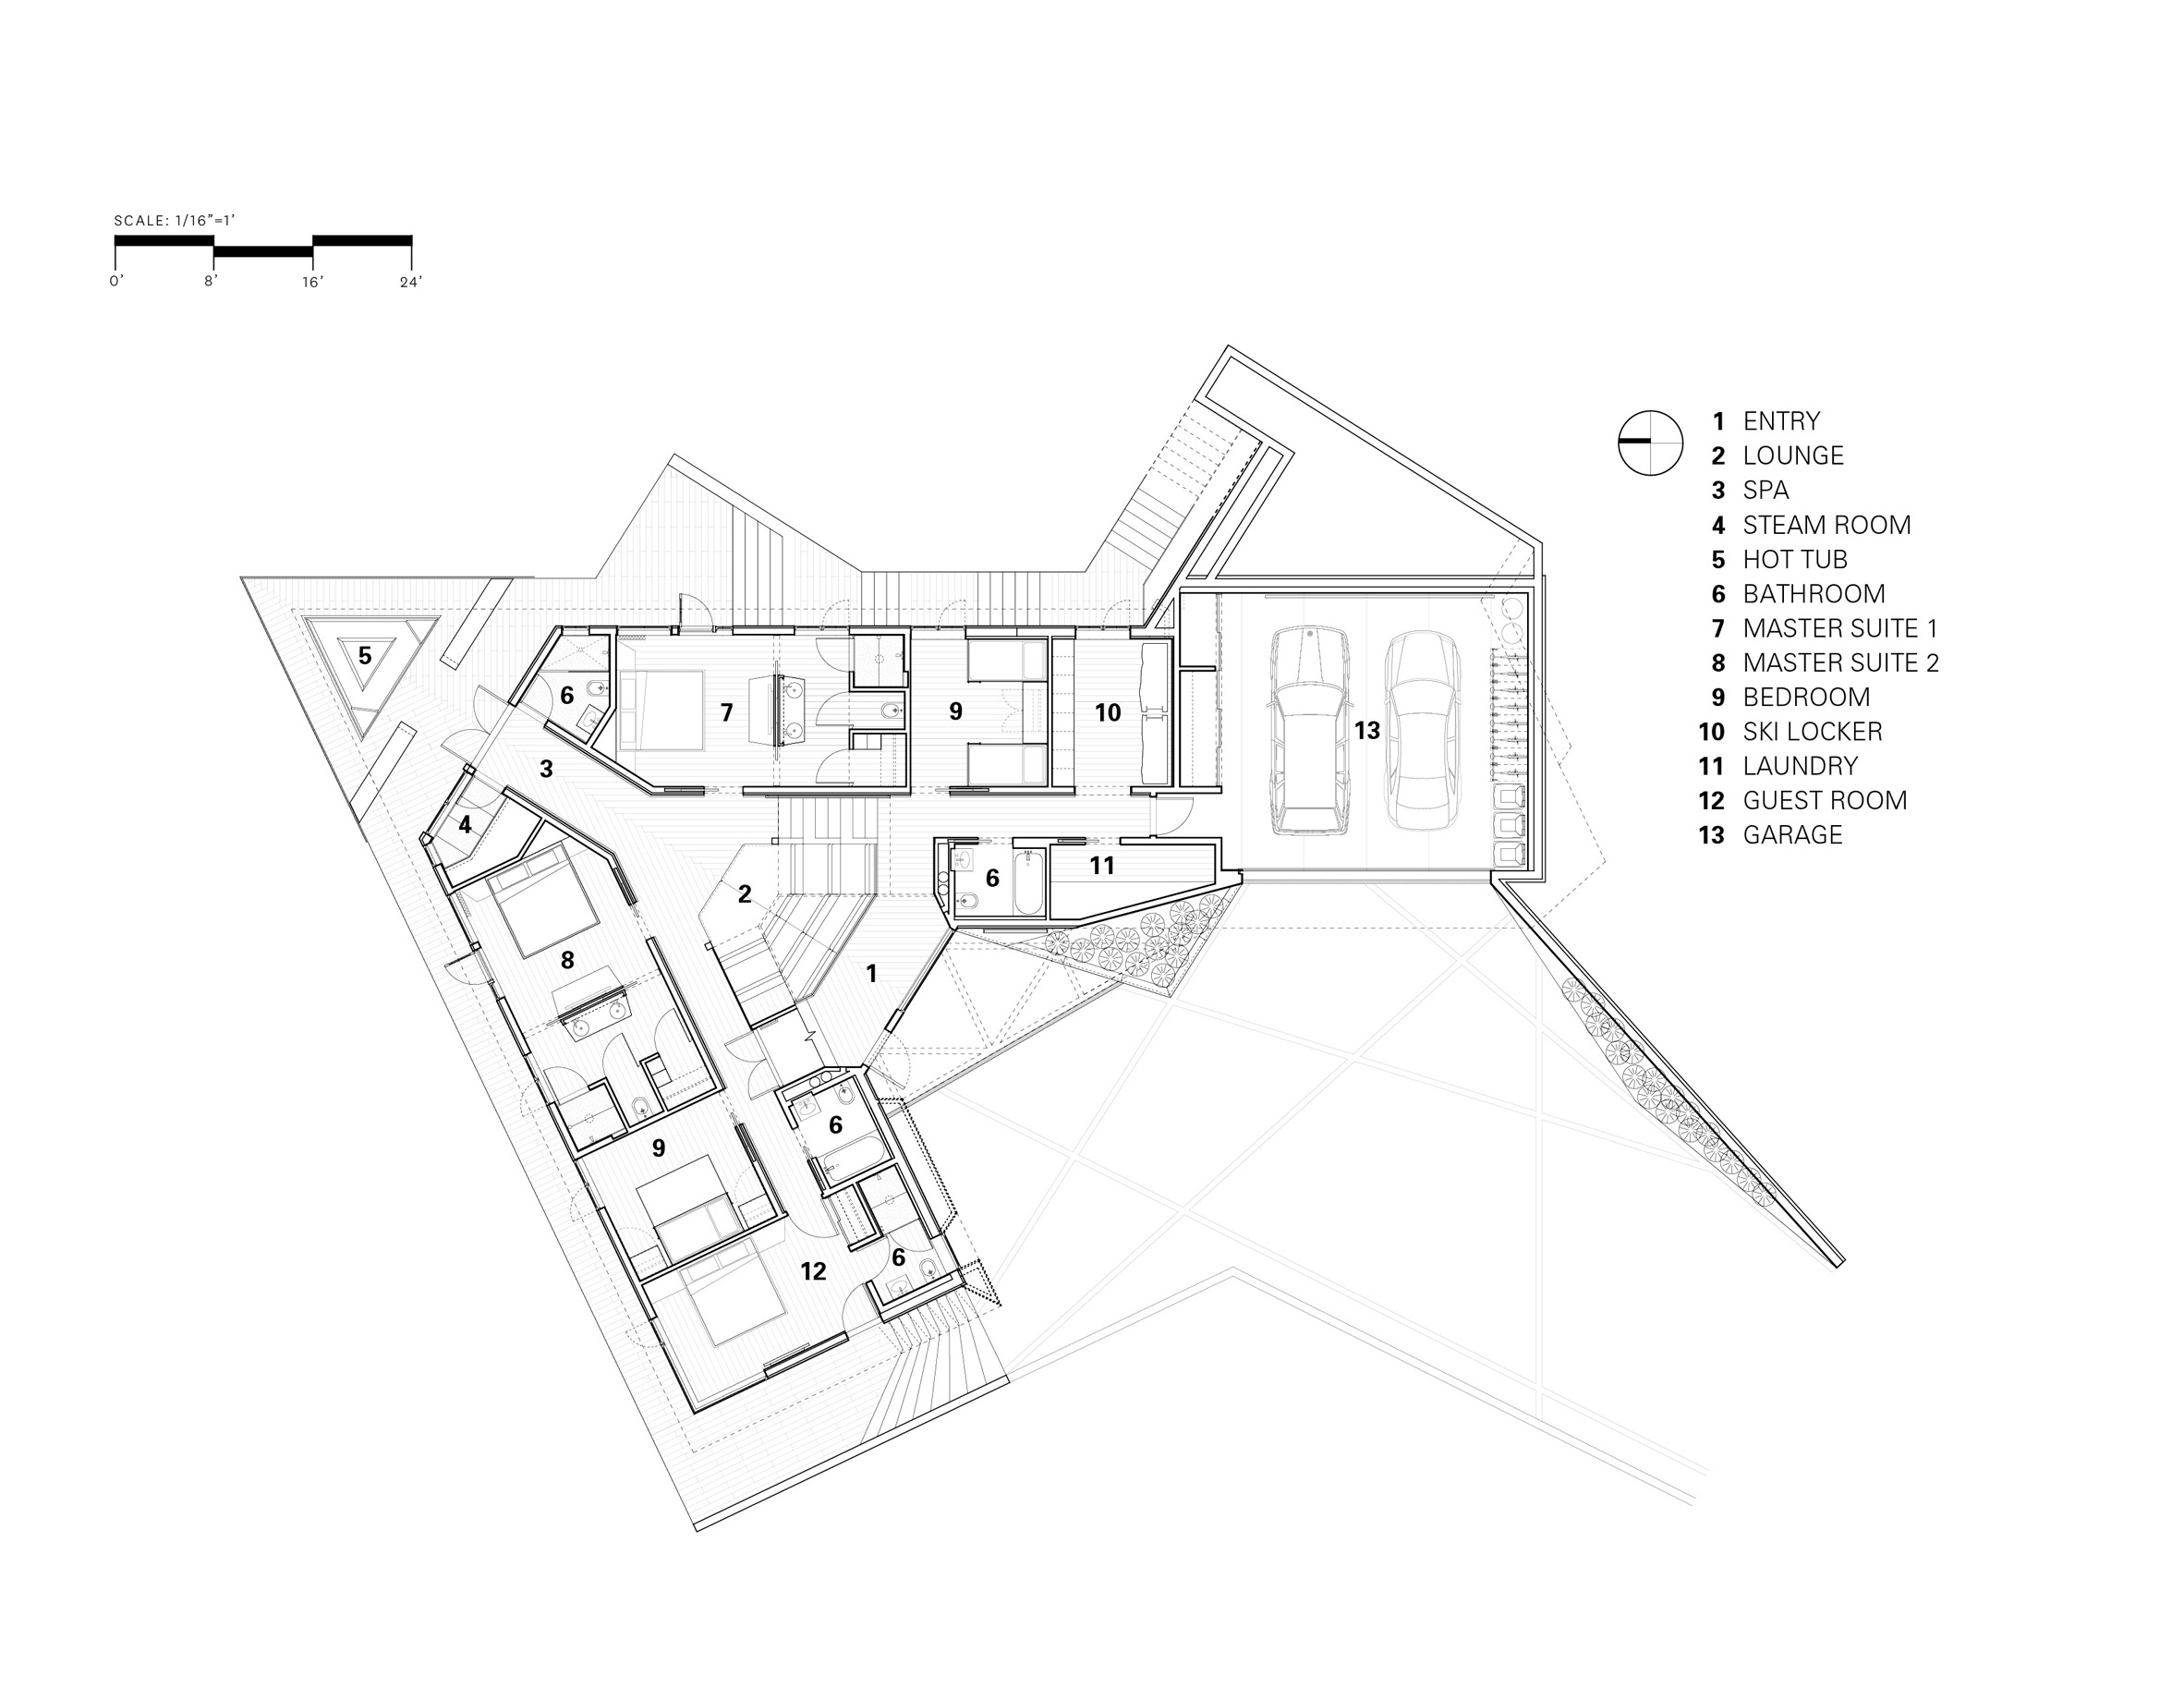
\includegraphics[width=1\textwidth]{fig/weird_floorplan.png}
    \label{}
    \caption[Weird floor plan]{Weird floor plan~\cite{weird_building}}
\end{figure}

When using a grid system apporach it will be possible to get an agent to walk from area 12 to 13 by specifically telling it which nodes are walkable and which nodes are not e.g walls. This will not be possible for the graph connectivity graph. The graph will here see only that area 12 and 13 are connected but not in which way. The method will draw a straight line between the two points and not see that the areas in reality are connected by the long pathway that goes through the entire floor plan.


\subsection{Grid system paper}
In this paper \cite{xu2017bim} they have the goal of solving “Accurate and efficient indoor path planning” in BIM models. The way they have implemented it is by using the grid system. 

\begin{figure}[H]
    \centering
    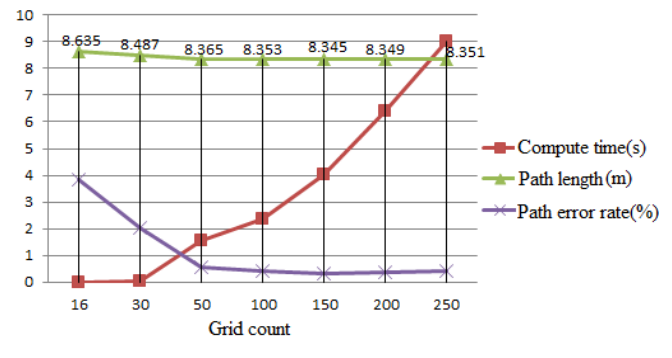
\includegraphics[width=1\textwidth]{fig/graph_grid_system.PNG}
    \caption{Graph showing computation cost as a function of grid count~\cite{xu2017bim}}
    \label{}
\end{figure}

They show what happens with the computation time when increasing the number of nodes. And also shows how minimal an effect it has on the path length.

Skriv om Convex decomposition vs alternativer(K means)

\\\\
\subsection{Conclusion}
blabal


\subsection{Future work}
You can write about slam
Write about stairs
Write about the whole thing about actually getting the robot to traverse the route and programming the robot
\end{comment}